\documentclass[preprint,authoryear,11pt]{report}
\setlength{\parindent}{0cm}
\usepackage{titlesec}
\usepackage{lipsum}
\usepackage{booktabs}% http://ctan.org/pkg/booktabs
\usepackage{colortbl}% http://ctan.org/pkg/colortbl
\usepackage{amsmath}% http://ctan.org/pkg/amsmath
\usepackage{xcolor}% http://ctan.org/pkg/xcolor
\usepackage{graphicx}% http://ctan.org/pkg/graphicx
\usepackage{amsmath}
\usepackage{subcaption}
\usepackage{amsthm}
\usepackage{amssymb}
\usepackage{graphicx}
\usepackage[margin=1.5in]{geometry}
\usepackage{pdflscape}
\usepackage{palatino}
\usepackage{hyperref}
\usepackage{natbib}
\usepackage{titlepic}
\usepackage{graphicx}
\usepackage{setspace}
\usepackage{float}
\usepackage{verbatim}
\usepackage{tikz}
\usetikzlibrary{snakes}
%\usepackage[framed]{mcode}
\usepackage{amsmath,varwidth,array,ragged2e}
\newcolumntype{L}{>{\varwidth[c]{\linewidth}}l<{\endvarwidth}}
\newcolumntype{M}{>{$}l<{$}}
\def\ds{\mathrm{d}s}%
\usepackage{units}
\newcommand{\E}{\mathbb{E}}
\newcommand{\Sa}{\sum_{i=1}^d}
\newcommand{\Mx}{M_{X_{i}}(d)}
\newcommand{\MX}{M_{\underline{X}}(\underline{1})}
\newcommand{\EL}{\E\left[l(\mathrm{\underline{X}}-\underline{m})\right]}
\newcommand{\EdL}{\E\left[\frac{\partial}{\partial x_i}l(\mathrm{\underline{X}}-\underline{m})\right]}
\newcommand{\nla}{\\ \Rightarrow \,}
\newcommand{\Xun}{\mathrm{\underline{X}}}  

\graphicspath{ {images/} }
\usepackage{xcolor}
\usepackage{lipsum}% Used for dummy text.
\definecolor{titlepagecolor}{cmyk}{1,.60,0,.40}
\definecolor{namecolor}{cmyk}{1,.50,0,.10} 

% Theorem declarations
\theoremstyle{definition}
\newtheorem{theorem}{Theorem}[section]
\newtheorem{definition}[theorem]{Definition}
\newtheorem{proposition}[theorem]{Proposition}
\newtheorem{lemma}[theorem]{Lemma}
\newtheorem{corollary}[theorem]{Corollary}
\newtheorem{remark}[theorem]{Remark}
\newtheorem{example}[theorem]{Example}


\newcommand{\Ainfo}{\mathcal{A}}
\newcommand{\Afiltration}{\underline{\mathcal{A}}}
\newcommand{\real}{\mathfrak{R}}
\newcommand{\naturalNum}{\mathcal{N}}
\newcommand{\normalDist}{\mathcal{N}}
\newcommand{\rnQ}{\mathbb{Q}}
\newcommand{\forward}{\text{For}}
\newcommand{\future}{\text{Fut}}
\newcommand{\variance}{\mathbb{V}\text{ar}}
\newcommand{\covariance}{\mathbb{C}\text{ov}}
\newcommand{\indicator}{\mathbb{I}}
\newcommand{\bigO}{\mathcal{O}}
\newcommand{\cadlag}{c\`{a}dl\`{a}g\ }
\renewcommand\thesection{\arabic{section}}

\providecommand{\abs}[1]{\lvert#1\rvert}
\providecommand{\norm}[1]{\lVert#1\rVert}

% The following commands are for better float positioning (http://mintaka.sdsu.edu/GF/bibliog/latex/floats.html)
%   General parameters, for ALL pages:
\renewcommand{\topfraction}{0.9}          % max fraction of floats at top
\renewcommand{\bottomfraction}{0.8}       % max fraction of floats at bottom
%   Parameters for TEXT pages (not float pages):
\setcounter{topnumber}{2}
\setcounter{bottomnumber}{2}
\setcounter{totalnumber}{4}               % 2 may work better
\setcounter{dbltopnumber}{2}              % for 2-column pages
\setcounter{secnumdepth}{3}
\setcounter{tocdepth}{3}
\renewcommand{\dbltopfraction}{0.9}       % fit big float above 2-col. text
\renewcommand{\textfraction}{0.07}        % allow minimal text w. figs
%   Parameters for FLOAT pages (not text pages):
\renewcommand{\floatpagefraction}{0.7}    % require fuller float pages
% N.B.: floatpagefraction MUST be less than topfraction !!
\renewcommand{\dblfloatpagefraction}{0.7} % require fuller float pages
% remember to use [htp] or [htpb] for placement
\newcommand*{\plogo}{\fbox{$\mathcal{PL}$}} % Generic publisher logo

\setlength{\parindent}{1em}
\setlength{\parskip}{1em}

\colorlet{tableheadcolor}{gray!25} % Table header colour = 25% gray
\newcommand{\headcol}{\rowcolor{tableheadcolor}} %
\colorlet{tablerowcolor}{gray!10} % Table row separator colour = 10% gray
\newcommand{\rowcol}{\rowcolor{tablerowcolor}} %
    % Command \topline consists of a (slightly modified) \toprule followed by a \heavyrule rule of colour tableheadcolor (hence, 2 separate rules)
\newcommand{\topline}{\arrayrulecolor{black}\specialrule{0.1em}{\abovetopsep}{0pt}%
            \arrayrulecolor{tableheadcolor}\specialrule{\belowrulesep}{0pt}{0pt}%
            \arrayrulecolor{black}}
    % Command \midline consists of 3 rules (top colour tableheadcolor, middle colour black, bottom colour white)
\newcommand{\midline}{\arrayrulecolor{tableheadcolor}\specialrule{\aboverulesep}{0pt}{0pt}%
            \arrayrulecolor{black}\specialrule{\lightrulewidth}{0pt}{0pt}%
            \arrayrulecolor{white}\specialrule{\belowrulesep}{0pt}{0pt}%
            \arrayrulecolor{black}}
    % Command \rowmidlinecw consists of 3 rules (top colour tablerowcolor, middle colour black, bottom colour white)
\newcommand{\rowmidlinecw}{\arrayrulecolor{tablerowcolor}\specialrule{\aboverulesep}{0pt}{0pt}%
            \arrayrulecolor{black}\specialrule{\lightrulewidth}{0pt}{0pt}%
            \arrayrulecolor{white}\specialrule{\belowrulesep}{0pt}{0pt}%
            \arrayrulecolor{black}}
    % Command \rowmidlinewc consists of 3 rules (top colour white, middle colour black, bottom colour tablerowcolor)
\newcommand{\rowmidlinewc}{\arrayrulecolor{white}\specialrule{\aboverulesep}{0pt}{0pt}%
            \arrayrulecolor{black}\specialrule{\lightrulewidth}{0pt}{0pt}%
            \arrayrulecolor{tablerowcolor}\specialrule{\belowrulesep}{0pt}{0pt}%
            \arrayrulecolor{black}}
    % Command \rowmidlinew consists of 1 white rule
\newcommand{\rowmidlinew}{\arrayrulecolor{white}\specialrule{\aboverulesep}{0pt}{0pt}%
            \arrayrulecolor{black}}
    % Command \rowmidlinec consists of 1 tablerowcolor rule
\newcommand{\rowmidlinec}{\arrayrulecolor{tablerowcolor}\specialrule{\aboverulesep}{0pt}{0pt}%
            \arrayrulecolor{black}}
    % Command \bottomline consists of 2 rules (top colour
\newcommand{\bottomline}{\arrayrulecolor{white}\specialrule{\aboverulesep}{0pt}{0pt}%
            \arrayrulecolor{black}\specialrule{\heavyrulewidth}{0pt}{\belowbottomsep}}%
\newcommand{\bottomlinec}{\arrayrulecolor{tablerowcolor}\specialrule{\aboverulesep}{0pt}{0pt}%
            \arrayrulecolor{black}\specialrule{\heavyrulewidth}{0pt}{\belowbottomsep}}%


%----------------------------------------------------------------------------------------
%	TITLE PAGE
%----------------------------------------------------------------------------------------

\newcommand*{\titleGM}{\begingroup % Create the command for including the title page in the document
\hbox{ % Horizontal box
\hspace*{0.2\textwidth} % Whitespace to the left of the title page
\rule{1pt}{\textheight} % Vertical line
\hspace*{0.05\textwidth} % Whitespace between the vertical line and title page text
\parbox[b]{0.75\textwidth}{ % Paragraph box which restricts text to less than the width of the page

\begin{flushleft}
{\noindent\Huge\bfseries A metamodelling approach to estimate fair market values}\\[2\baselineskip] % Title
\end{flushleft}
{\large \textit{TEAM BIGS}}\\[ \baselineskip] % Team number
{\large{\textsc{Brenda Prallon}}, \small{EMAp-FGV} \\ \large{\textsc{Gabriel Novais}}, \small{EMAp-FGV}\\ \large{\textsc{Igor Carvalho}}, \small{EMAp-FGV}} \\ \large{\textsc{Sergio Maffra}}, \small{King's College London} \\ % Author name and affiliated university
{\large{\textsc{\\\textit{Supervisor}}}: \\ \large{\textsc{Emiliano Valdez}}, \small{University of Connecticut} \\ } % Mentor and affiliated company/university

\vspace{80mm} % Whitespace between the title block and the publisher
{\noindent \small{EMAp, Funda\c{c}\~ao Getulio Vargas, Rio de Janeiro, Brazil}}\\[\baselineskip] % Publisher and logo
}}
\endgroup}

\begin{document}
	\restoregeometry % restores the geometry
	\nopagecolor % Use this to restore the color pages to white
 \thispagestyle{empty} % Removes page numbers

\titleGM 

\begingroup
	\makeatletter
	% Redefine the \chapter* header macro to remove vertical space
	\def\@makeschapterhead#1{%
	  %\vspace*{50\p@}% Remove the vertical space
	  {\parindent \z@ \raggedright
	    \normalfont
	    \interlinepenalty\@M
	    \Huge \bfseries  #1\par\nobreak
	    \vskip 40\p@
	  }}
	\makeatother

\endgroup

\tableofcontents

\chapter{Introduction}

A variable annuity (VA) is a life insurance product created by insurance companies to address concerns that many people have about outliving their assets. Essentially, a VA is a deferred annuity with two phases: the accumulation phase and the payout phase. During the accumulation phase, the policyholder makes purchase payments to the insurance company. During the payout phase, policyholders receive benefit payments from the insurance company. The policyholder has the option of allocating his investments among a set of investment funds. 

A major feature of a variable annuity is that it includes guarantees or riders. These can be divided into two broad categories: death benefits and living benefits. A guaranteed minimum death benefit (GMDB) guarantees a specified lump sum to the beneficiary upon the death of the policyholder regardless of the performance of the investment portfolio. There are several types of living benefits, which include the guaranteed minimum withdrawal benefit (GMWB), the guaranteed minimum income benefit (GMIB), the guaranteed minimum maturity benefit (GMMB), and the guaranteed minimum accumulation benefit (GMAB). A GMWB guarantees that policyholders can make systematic annual withdrawals of a specified amount from the benefit base over a period of time, even though the investment portfolio might be depleted. A GMIB guarantees that policyholders can convert the greater of the current account value or the benefit base to an annuity according to a specified rate. A GMMB guarantees that policyholders received a specific amount at the maturity of the contract. A GMAB guarantees that policyholders can renew the contract during a specified window after a specified waiting period (usually 10 years).

\begin{figure}
  	\begin{subfigure}[b]{0.5\textwidth}
    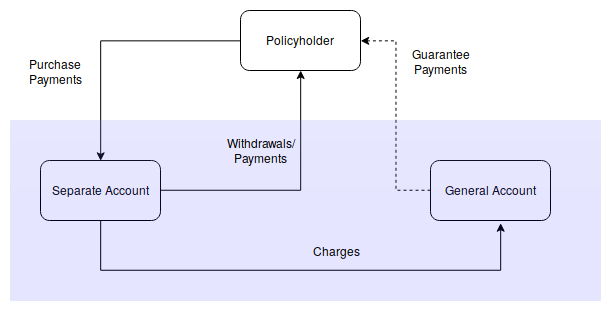
\includegraphics[width=\textwidth]{pictures/novais1.png}
    \caption{Variable annuity flowchart}
    \label{fig:1}
  	\end{subfigure}
  	%
  	\begin{subfigure}[b]{0.5\textwidth}
    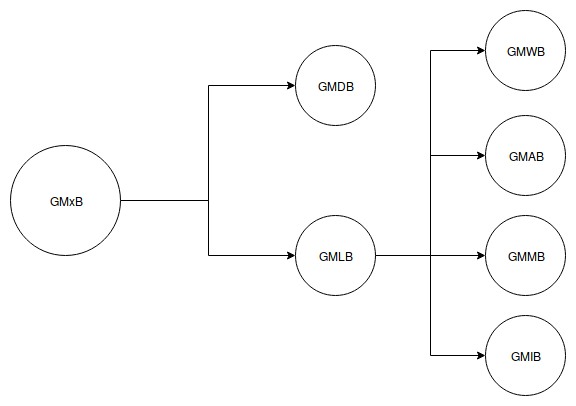
\includegraphics[width=\textwidth]{pictures/novais2.png}
    \caption{Guarantees}
    \label{fig:2}
  	\end{subfigure}
  	\caption{Variable Annuities Description}
\end{figure}


Using dynamic hedging to mitigate the financial risks associated with VA guarantees, insurance companies need to estimate the fair market value (FMV) of guarantees for a large portfolio of VA contracts in a timely manner. 
%Dynamic hedging requires calculating the dollar Deltas of a portfolio of variable annuity policies within a short interval. 
As the value of the guarantees cannot be determined by closed-form formulas, Monte Carlo (MC) simulations are used to value VA portfolios. This approach can be extremely time-consuming as every contract needs to be projected over many scenarios for a long time horizon. To address this computational problem, metamodeling approaches have been proposed.

Metamodeling approaches can significantly reduce the computational effort in the valuation of a large portfolio of VA contracts for two main reasons: first, only a small group of representative contracts needs to be valued using Monte Carlo simulations; second, metamodels are usually simpler and faster than Monte Carlo simulation models. The basic four steps to build a metamodel are illustrated in Figure~\ref{metamodeling}. They consist in: (1) defining a subset of representative VA contracts, (2) computing the FMV for this representative set using MC simulations, (3) fitting a model based on the characteristics and FMV of the contracts, (4) using the estimated model to predict the FMV of the remaining VA contracts. 

\begin{figure}[ht]
\begin{center}
  	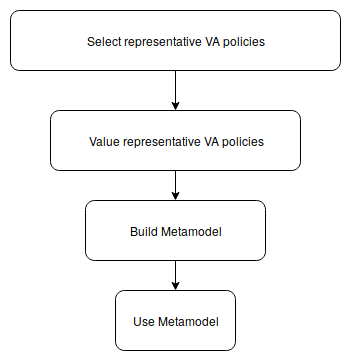
\includegraphics[width=0.4\textwidth]{pictures/novais3.png}
    \caption{Metamodel fluxogram}\label{metamodeling}
\end{center}
\end{figure}




%\chapter{Review}

%The metamodels investigated in literature are sophisticated predictive models, which might cause difficulties in terms of interpretation or calibration.

%There are many publications on metamodeling approaches, which are, essentially, sophisticated predictive models. 
%Recently, these approaches have been used to speed up the valuation of large VA portfolios. 
Table~\ref{tab:metamodeling} shows the main metamodeling approaches applied in the valuation of VA portfolios. Some of the metamodels proposed include: linear regression models with interactions, GB2 regression model, ordinary kriging, universal kriging,  rank-order kriging (quantile kriging), and tree-based models.  

\cite{gan2018valuation} investigated the effect of including interactions in linear regression models for the valuation of large VA portfolios. His results show that including interactions in linear regression models can lead to significant improvements in prediction accuracy. 
%Since VA contracts have many features, a large number of possible interactions might exist between them. So he selected the important interactions using overlapped group-lasso that could produce hierarchical interaction models. The numeric results obtained in \cite{gan2018valuation} show that including interactions in linear regression models can lead to significant improvements in prediction accuracy. 

In \cite{gan2017modeling}, the GB2 distribution was used to model the fair market values of VA guarantees, because it can capture the skewness found in their empirical distributions. 
%The GB2 distribution is a flexible statistical distribution that contains three shape parameters and one scale parameter. 
%However, finding the optimum parameters for the GB2 regression model was not straightforward and therefore difficult numerical challenges were present. 
The numerical results of the approach show that the four-stage optimization, described in the article, performs well and the fitted GB2 regression model performed as expected. A few comparisons made by the authors: (1) the GB2 model captures skewness better than the kriging model; (2) the GB2 model outperforms the kriging model in computational speed; (3) GB2 model produces comparably accurate predictions as the kriging model at portfolio level.

An important step in the metamodeling process is the selection of representative policies. Gan and Valdez (2016) compared five different experimental design methods for the GB2 regression model: random sampling, low-discrepancy sequence, data clustering (hierarchical k-means), Latin hypercube sampling, and conditional Latin hypercube sampling.

\cite{hejazi2016neural} proposed a machine learning approach. After a small set of representative VA contracts was selected and valued via Monte Carlos simulations, the values of these representatives contracts were then used in a spatial interpolation method that found the value of the contracts in the input portfolio as a linear combination of the values of the representative contracts. The traditional spatial interpolation methods as kriging, IDW and RBF (Hejazi 2015) have a strong dependence on the distance function used in estimations. Therefore, the authors proposed a neural network implementation of the spatial interpolation technique that learns an effective choice of distance function. The results show the superior accuracy of the neural network approach in estimation of the delta value for the input portfolio when compared to the traditional spatial interpolation techniques.

\cite{xu2018moment} propose a moment matching machine learning (MMML) approach to compute dollar deltas, VaRs and CVaRs for large portfolios. There are two main contributions that could be highlighted in their paper. First, they proposed a moment matching method for single VA contracts. Computations using this method are much faster than nested MC simulations.
%
%Due to these selected scenarios, the moment matching method can compute the annual dollar deltas, VaRs and CVaRs as accurately as the nested simulations, but takes far less computational time then nested simulations. 
%
The second contribution is that they combine the moment matching method with classical machine learning methods to manage the risk of large VA portfolios. 
%The ``machine is trained'' with a standard machine learning method, such as neural network or tree regressions. 
%Their MMML approach can easily handle large portfolios (which cannot be handled via the nested simulation method due to cost). Their approach appears to be a remarkably efficient alternative to the standard nested simulation methodology to hedge and manage the risk of large portfolios arising in the insurance industry.
Their MMML approach can easily handle large portfolios, being a remarkably efficient alternative to the standard nested simulation methods to hedge and manage the risk of large portfolios arising in the insurance industry.


\begin{table}
\begin{center}
\begin{small}
\makebox[\textwidth][c]{
\begin{tabular}{lll}
\toprule
Publication & Experimental Design & Metamodel \\
\midrule
Gan (2013) & Clustering & Kriging \\
Gan and Lin (2015) & Clustering & Kriging \\
Gan (2015) & LHS & Kriging \\
Hejazi and Jackson (2016) & Uniform sampling & Neural network \\
Gan and Valdez (2016) & Clustering, LHS & GB2 regression \\
Gan and Valdez (2017) & Clustering & gamma regression \\
Gan and Lin (2017) & LHS, conditional LHS & Kriging \\
Hejazi et al. (2017) & Uniform sampling & Kriging, IDW, RBF\\
Gan and Huang (2017) & Clustering & Kriging \\
Xu et al (2018) & Random sampling & Neural Network, regression trees \\
Gan and Valdez (2018) & Clustering & GB2 regression \\
Quan, Gan and Valdez (2019) & Clustering & Regression trees \\
\bottomrule
\end{tabular}
}
\end{small}
\end{center}
\caption{Metamodeling approaches for the valuation of variable annuities.}\label{tab:metamodeling}
\end{table}




\chapter{The synthetic data set}\label{chap:dataset}

Researchers usually do not have access to real data sets from insurance companies. As a result, most of the papers on the valuation of variable annuity portfolios rely on synthetic data sets to test the performance of the proposed techniques. To assist in the development and dissemination of research related to the efficient valuation of large variable annuity portfolios, \cite{gan2017modeling} created synthetic data sets that are based on the properties of real portfolios of variable annuities. They have also implemented a simple Monte Carlo valuation engine that is used to calculate the fair market value and the Greeks of the guarantees embedded in the synthetic variable annuity contracts.

%The main properties typically observed on real portfolios of variables annuities contracts are:
Contracts found in real portfolios of variable annuities are typically characterized by having different types of guarantees, different investment fund allocations, and different issue and maturity dates.
%\begin{itemize}
%\item Different contracts may contain different types of guarantees.
%\item The contract holder has the option to allocate his investments among multiple investment funds.
%\item Real variable annuity contracts are issued at different dates and have different times to maturity.
%\end{itemize}
%
To account for the different types of guarantees, % typically present in a VA contract, 
%There are several types of guarantees, but to create a synthetic portfolio of variable annuity contracts, 
\cite{gan2017modeling} consider the 19 products shown in Table~\ref{tab:prods}. 
%For the synthetic variable annuity policies, they set rider fees of individual riders in the range of 0.25\% to 0.75\%. The rider fee of the combined guarantees is equal to the sum of the fees of the individual guarantees minus 0.20\%.
Rider fees are set in the range of 0.25\% to 0.75\%, and the rider fee of the combined guarantees is equal to the sum of individual ones minus 0.2\%.
%
%In dynamic hedging, 
The investment choices of a policyholder are mapped to a combination of tradable and liquid indices such as the S\&P500 index. In the synthetic portfolio, account values of the investment funds were generated randomly from a specified range and allocated to investment funds in equal proportions. 
%
In practice, variable annuity policies in a portfolio are issued at different dates. To value the policies at the valuation date, the policies are aged from the issue dates to the valuation date. Finally, the parameters used to generate others variables, such as time to maturity and age come from the variables displayed in Table~\ref{tab:params}.

\begin{table}
\begin{center}
\begin{small}
\begin{tabular}{l l l}
\toprule
Product & Description                 & Rider Fee  \\
\midrule
DBRP    & GMDB with return of premium & 0.25\%     \\
DBRU    & GMDB with annual roll-up     & 0.35\%     \\
DBSU    & GMDB with annual ratchet     & 0.35\%     \\
ABRP    & GMAB with return of premium & 0.50\%     \\
ABRU    & GMAB with annual roll-up     & 0.60\%     \\
ABSU    & GMAB with annual ratchet     & 0.60\%     \\
IBRP    & GMIB with return of premium & 0.60\%     \\
IBRU    & GMIB with annual roll-up     & 0.70\%     \\
IBSU    & GMIB with annual ratchet     & 0.70\%     \\
MBRP    & GMMB with return of premium & 0.50\%     \\
MBRU    & GMMB with annual roll-up     & 0.60\%     \\
MBSU    & GMMB with annual ratchet     & 0.60\%     \\
WBRP    & GMWB with return of premium & 0.65\%     \\
WBRU    & GMWB with annual roll-up     & 0.75\%     \\
WBSU    & GMWB with annual ratchet     & 0.75\%     \\
DBAB    & GMDB + GMAB with annual ratchet & 0.75\%     \\
DBIB    & GMDB + GMIB wwith annual ratchet     & 0.85\%     \\
DBMB    & GMDB + GMMB with annual ratchet     & 0.75\%     \\
DBWB    & GMDB + GMWB with annual ratchet & 0.90\% \\
\bottomrule
\end{tabular}
\end{small}
\end{center}	
\caption{Variable annuity products in the synthetic database.}\label{tab:prods}
\end{table}
	

\begin{table}
\begin{small}
\begin{center}
\begin{tabular}{l l l}
\toprule
Feature & Value \\
\midrule
Policyholder birth date & [1/1/1950,1/1/1980] \\
Issue date & [1/1/2000,1/1/2014] \\
Valuation date & 1/6/2014 \\
Maturity & [15,30]years \\
Initial account value & [50000,500000] \\
Female percent & 40\% \\
Fund fee & 30, 50, 60, 80, 10, 38, 45, 55, 57, 46 bps for Funds 1 to 10 \\
M\&E fee & 200 bps \\
\bottomrule
\end{tabular}
\caption{Parameters used in the generation of the synthetic database of variable annuities.}\label{tab:params}
\end{center}
\end{small}
\end{table}

%There are two types of scenarios: risk-neutral and real-word. Each of these two scenarios are generated by each measures respectively. Risk-neutral scenarios are used to calculate the fair market values of financial derivatives such as the guarantees embedded in variable annuities. Real-world scenarios are used to calculate solvency capitals or evaluate hedging strategies.

 The data sets generated by \cite{gan2017modeling} contain 10,000 synthetic variable annuity policies for each of the guarantees types described in Table~\ref{tab:prods}. Therefore, the synthetic portfolio contains 190,000 policies. There are 45 fields in each policy, including 10 fund values, 10 fund numbers and 10 fund fees. The description of the policy fields in the synthetic data set is shown in Table~\ref{tab:fields}.

\begin{table}
\begin{center}
\begin{small}
\begin{tabular}{l l l}
\toprule
Field & Description \\
\midrule
recordID & Unique identifier of the policy \\
survivorShip & Positive weighting number\\
gender & Gender of the policyholder \\
productType & Product type \\
issueDate & Issue Date \\
matDate & Maturity date\\
birthDate & Birth date of the policyholder \\
currentDate & Current date\\
baseFee & M\&E (Mortality \& Expense) fee \\
riderFee & Rider fee \\
rollUprate & Roll-up rate\\
rollUprate & Guaranteed benefit\\
rollUprate & GMWB balance\\
wbWithdrawalRate & Guaranteed withdrawal rate\\
withdrawal & Withdrawal so far\\
FundValuei & Fund value of the ith investment fund\\
FundNumi & Fund number of the ith investment fund\\
FundFeei & Fund management fee of the ith investment fund\\
\bottomrule
\end{tabular}
\end{small}
\end{center}
\caption{Description of fields in the specification of variable annuities policies.}\label{tab:fields}
\end{table}

The main goal of Monte Carlo simulation engine is calculate the fair market values (FMV), partial dollar deltas and partial dollar rhos of the guarantees for the synthetic portfolios. Total fair market values are usually positive, as guarantee benefit payoffs are larger than their associated risk. Since the VA contracts are usually long-terms contracts, guarantees are more sensitive to long-term interest rates than to short-term interest rates. 

%The total amount of those variables are described above: 

%\begin{table}
%\begin{small}
%\begin{center}
%\begin{tabular}{l l l l}
%\hline
%Quantity Name & Value & Quantity Name & Value  \\
%\hline
%FMV & 18,572,095,089 & Rho2y & 167,704 \\
%Delta1 & -4,230,781,199 & Rho3y & 85,967 \\
%Delta2 & -2,602,768,996 & Rho4y & 2,856 \\
%Delta3 & -2,854,233,170 & Rho5y & -96,438 \\
%Delta4 & -2,203,726,514 & Rho7y & 546,045 \\
%Delta5 & -2,341,793,581 & Rho10y & 1,407,669 \\
%Rho1y & 40,479 & Rho30y & 62,136,376 \\
%\hline
%\end{tabular}
%\end{center}
%\end{small}
%\caption{Example of variable annuity contract.}
%\end{table}


%\begin{table}
%\begin{small}
%\begin{center}
%\begin{tabular}{l l l l}
%\toprule
%Quantity Name & Value\\
%\midrule
%FMV & 18,572,095,089 \\
%Delta1 & -4,230,781,199 \\ 
%Delta2 & -2,602,768,996 \\ 
%Delta3 & -2,854,233,170 \\
%Delta4 & -2,203,726,514 \\ 
%Delta5 & -2,341,793,581 \\ 
%Rho1y & 40,479 \\ 
%Rho2y & 167,704 \\
%Rho3y & 85,967 \\
%Rho4y & 2,856 \\
%Rho5y & -96,438 \\
%Rho7y & 546,045 \\
%Rho10y & 1,407,669 \\
%Rho30y & 62,136,376 \\
%\bottomrule
%\end{tabular}
%\end{center}
%\end{small}
%\caption{Example of variable annuity contract.}
%\end{table}

\chapter{The challenge}
\section{Problem statement}

%The valuation of variable annuity portfolios consists in a prediction problem. The scope of this work is to investigate interaction terms in the Generalized Linear Model framework as a metamodel for the valuation of the complex financial guarantees associated with VA contracts. %Althought its very important accuracies and variances in prediction models, we would also like to interpret how the characteristics of the contracts affect their fair market values.

%The Overlapped Grouped Lasso approach produce residuals from regression that are not normally distributed, hence we cannot interpret p-values as significant. There is a possible solution that concerns to applying the GLM with Overlapped Group Lasso to model the problem. In order to solve this we propose  Box-Cox regression model, which can handle with those  not normally distributed residuals by introducing some transformations. Others possibilities to deal with the prediction problem without concern with these residuals is just look to machine learning metamodels as Tree Based regression and Neural Network model.

The objective of the project is to improve the consistency in the determination of statistically significant interaction terms in linear models with interactions used for the valuation of portfolios of variable annuity contracts. The approach has been introduced in~\cite{gan2018regression} with excellent prediction results. However, the non-Gaussian residuals of the fitted models compromise any inference based on the hypothesis of gaussianity. Consequently, one cannot identify the significant interaction terms and interpret the predictions provided by the models.

Initially, an investigation of interaction terms in the framework of generalized linear models was considered. However, given the time constraints of the challenge, other alternative solutions were explored. First, as described in Section~\ref{sec:linear_model}, we replicate the results obtained in~\cite{gan2018regression} as a starting point. In the following section, we explore the Box-Cox regression model as an alternative to improve the original results. Finally, in Section~\ref{sec:tree_based_models}, we explore tree-based models as a metamodeling approach, as in~\cite{quan2018tree}.

%		 \begin{frame}{The Problem}
%        \begin{itemize}
%			\setlength\itemsep{0,7em}    
%            \item The valuation of variable annuity portfolios: a prediction problem;
%            \item But we would also like to interpret how the characteristics of the contracts affect their fair market values;
%            \item The Overlapped Grouped Lasso: the residuals of the regression are not normally distributed, hence we cannot interpret p-values as %significant;
%            \item Possible solution: GLM with Overlapped Group Lasso;
%            %\item Issue: algorithm is not implemented in any package and involves multiple step optimizatio;
%            \item Proposed solution: Box-Cox regression model.
%       	 \end{itemize}
%    	\end{frame}		
%		\begin{itemize}
%			\setlength\itemsep{0,5em}
%			\item The scope of this work is to investigate interaction terms in Generalized Linear
%Model framework as a metamodel for valuing the complex financial guarantees associated with VA contracts. 
%			\item We choose statiscally significant interaction terms to the model, evaluate performance as predictive model, and interpret the resulting effect of the addition of interaction terms. 
%			\item We propose others metamodels: Box Cox regression and Neural Network regression. After describe these methods we will compare both e suggest the best of them to evaluate a VA portfolio.
%		\end{itemize}

\section{Results}
%\chapter{Results}
\subsection{Linear models with interactions}\label{sec:linear_model}

%\frame {
%\frametitle{Linear models with interactions}
%\setbeamertemplate{itemize items}[ball]		
%Lasso
%\begin{itemize}
%	\setlength\itemsep{0,5em}
%	\item  Let $y = ( y_1 , y_2 , . . . , y_n )$ 0 denote the vector of responses and let X denote the design matrix. Then the lasso is defined as
%	\end{itemize}			 			 
%\begin{equation}
%\hat{\boldsymbol{\beta}}^{L A S S O}=\arg \min _{\boldsymbol{\beta}}\left(\frac{1}{2}\|\mathbf{y}-\mathbf{X} \boldsymbol{\beta}\|_{2}^{2}+\lambda\|\boldsymbol{\beta}\|_{1}\right)
%\end{equation}
%
%\;\;\;\;\;\;\centering where $\|\cdot\|_{2}$ denotes the $\ell^{2}$ -norm, $\|\cdot\|_{1}$ denotes the $\ell^{1}$ -norm, and $\lambda$ is a tuning parameter that controls the amount of regularization.
%	  
%}
% \begin{block}{Interaction model}
%As mentioned earlier it was proposed different metamodeling approaches to compute the FMV of large VA portfolios.
% table $\#$ summarizes some of the main papers/metamodels dedicated to this task.

%\begin{figure}[h!]
%\makebox[\textwidth][c]{
%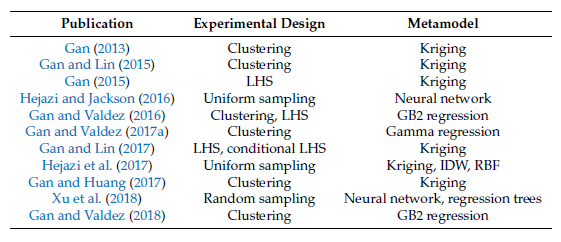
\includegraphics[scale=0.9]{pictures/some_approaches}
%}
%\end{figure}

% \textit{Include here the table 3 of paper: Valuation of large variable annuity portfolios using linear models with interactions}

%A brief look to the table above allow us verify that some approaches are quite sophisticated, e.g. kriging, neural network, GB2 regression. 

In this section, following \cite{gan2018valuation}, 
%it will be presented a linear regression model with interaction effects as an alternative method. 
a linear regression model with interaction effects is used in the valuation of VA contracts.
The main advantages of the approach discussed here is the simplicity in the metamodeling process, 
and the possibility of exploring interactions terms as features to predict the FMV of VA contracts. 

\subsubsection*{Interaction model}

% \vspace{0.25cm}
%By definition, an interaction exists between X and Y in a function $\textit{f}$ when $\textit{f}$ cannot be expressed as $g(x) + h(x)$, in other words, there are interactions when the response variable cannot be explained by additive function of the independent variables.
% \end{block}

By definition, interactions exist in a regression model when the response variable cannot be explained by additive functions of the independent explanatory variables.
%
%
Let $Y$ be a continuous response variable, and let $X_1, X_2, X_3, ..., X_n$ be the explanatory variables, including categorical and continuous, that will be used to model $Y$. The first-order interaction model can be write as:
% \vspace{0.5cm}

% \begin{block}{First order interaction model}
\begin{equation}
Y = \mu+\sum_{i=1}^{p} X_{i} \beta_{i}+\sum_{i<j} X_{i : j} \beta_{i : j} + \varepsilon,
\end{equation}

where the term $X_i$ denotes the individual effect of $X_i$ on $Y$; and $X_{i:j}$ denotes the effect of interaction between $X_i$ and $X_j$ on $Y$. In general lines, the equation (5.1) corresponds to an extension of the multiple linear regression model that is obtained with the inclusion of interaction terms.

The inclusion of interaction terms as explanatory variables can be viewed as the main virtue of the presented approach, since the added variables help to increase the predictive power of the model; however if the number of interaction terms to be included in the regression model is large, the estimated model can overfit the data. To avoid overfitting problem, two shrinkage methods are used to select the relevant interactions and estimate the parameters: group-LASSO and overlapped group-LASSO, to be presented in the next subsection.

% \begin{description}
% \item [$X_i$] main effect matrix
% %\item [$\beta_i$] main effect coefficient
% \item [$X_{i:j} $] interaction matrix
% %\item [$\beta_{i:j}$] main effect coefficient
% \end{description}
% \end{block}

% Types of interaction pairs:
% \begin{itemize}
%  \item categorical variables,
%  \item continuous variables,
%  \item categorical and continuous.
% \end{itemize}

% \begin{block}{Estimation of parameters}
\subsubsection*{Estimation of parameters}

Group-LASSO (GLASSO) and overlapped Group-LASSO (OGLASSO) can be considered general versions of the  LASSO,~\cite{tibshirani1996regression}. While the latter is designed for selecting individual input variables, GLASSO and OGLASSO are able to select important factors, or group of relevant variables.

Suppose that there are \textit{p} groups of variables. For $j = 1, 2, 3, ..., p$, let $\mathbf{X}_j$ denotes the feature matrix for group \textit{j}. The GLASSO can be formulated as:
% By solving the optimization problem
% \begin{equation}
% \hat{\beta}=\arg \min _{\beta} \left(\frac{1}{2}\left\|\mathbf{Y}-\mu \cdot \mathbf{1}-\sum_{i=1}^{p} \mathbf{X}_{i} \beta_{i}+\sum_{i<j} \mathbf{X}_{i : j} \beta_{i : j}\right\|_{2}^{2}\right)
% \end{equation}
% \end{block}
% \vspace{0.25cm}
% \begin{block}{Strong hierarchy}
% \vspace{0.25cm}
% Regularization techniques used to enforce \emph{strong hierarchy}.
% \end{block}
% \begin{block}{Lasso}
% \begin{equation}
% \hat{\boldsymbol{\beta}}^{L A S S O}=\arg \min _{\boldsymbol{\beta}}\left(\frac{1}{2}\|\mathbf{y}-\mathbf{X} \boldsymbol{\beta}\|_{2}^{2}+\lambda\|\boldsymbol{\beta}\|_{1}\right),
% \end{equation}
% %where $\lambda$ controls the amount of regularization.
% \end{block}
% \vspace{0.5cm}
% \begin{block}{Group-Lasso}
\begin{equation}
\hat{\beta}^{G L A S S O}=\arg \min _{\beta}\left(\frac{1}{2}\left\|\mathbf{y}-\beta_{0} \mathbf{1}-\sum_{j=1}^{p} \mathbf{X}_{j} \boldsymbol{\beta}_{j}\right\|_{2}^{2}+\lambda \sum_{j=1}^{p} \gamma_{j}\left\|\boldsymbol{\beta}_{j}\right\|_{1}\right),
\end{equation}
%where $X_{j}$ are feature groups and $\gamma_{j}$ are tuning parameters.
% \end{block}
where $\mathbf{1}$ is a vector of ones, $\left\| \bullet \right\|_2$ denotes the $\ell^{2}$-norm, and $\lambda, \gamma_1, ..., \gamma_p$ are tuning parameters. The parameter $\lambda$ controls the overall amount of regularization while the parameters $\gamma_1, ..., \gamma_p$ allow each group to be penalized to different extents. An attractive property of the GLASSO is that if $\boldsymbol{\hat{\beta_{j}}}$ is nonzero, then all of its components are typically nonzero.

% $\boldsymbol{\beta}$

In an intuitive way, GLASSO gives us the $\boldsymbol{\hat{\beta_j}}$ that minimize the mean squared error given a penalization term that shrinks parameters to zero. The selected group of variables are those related to the parameters that are nonzero. Optimal penalization terms can be chosen by cross-validation.

%\frame {
%\frametitle{Linear models with interactions}
%\setbeamertemplate{itemize items}[ball]		
%Group-Lasso
%\begin{itemize}
%	\setlength\itemsep{0,5em}
%	\item The group-lasso can be viewed as a general version of the popular Lasso.
%	\item Suppose that there are $p$ groups of variables. For $j=1,2, \ldots, p,$ let $X_{j}$ denote the feature matrix for group $j .$ The group-lasso can be formulated as follows:
%\end{itemize}			 			 
%\begin{equation}
%\hat{\beta}^{G L A S S O}=\arg \min _{\beta}\left(\frac{1}{2}\left\|\mathbf{y}-\beta_{0} \mathbf{1}-\sum_{j=1}^{p} \mathbf{X}_{j} \boldsymbol{\beta}_{j}\right\|_{2}^{2}+\lambda \sum_{j=1}^{p} %\gamma_{j}\left\|\boldsymbol{\beta}_{j}\right\|_{2}\right)
%\end{equation}
%
%\;\;\;\;\;\;\centering where 1 is a vector of ones, $\|\cdot\|_{2}$ denotes the $\ell^{2}$ -norm, and $\lambda, \gamma_{1}, \ldots, \gamma_{p}$ are tuning parameters.
%	  
%}

% \begin{block}{Overlapped Group-Lasso}
% \vspace{0.15cm}
% Group-Lasso with variables that can show up in different groups.
% \end{block}

The OGLASSO extends the GLASSO by adding an overlapped Group-LASSO penalty to the loss function in order to obtain hierarchical interaction models that can be formulated as the following unconstrained optimization problem:

% \begin{align*}
% \hat{\beta}^{O G L A S S O} &=\arg \min _{\beta}\left(\frac{1}{2}\left\|\mathbf{y}-\beta_{0} \mathbf{1}-\Sigma_{j=1}^{p} \mathbf{X}_{j} \beta_{j}-\sum_{s<t} \boldsymbol{X}_{s : t} \boldsymbol{\beta}_{s : t}\right\|_{2}^{2}\right. \\
% &+\lambda\left(\sum_{j=1}^{p}\left\|\boldsymbol{\beta}_{j}\right\|_{2}+\sum_{s<t}\left\|\boldsymbol{\beta}_{s : t}\right\|_{2}\right)\right)
% \end{align*}

\begin{align*}
\hat{\beta}^{O G L A S S O} =\arg \min _{\beta}\left(\frac{1}{2}\left\|\mathbf{y}-\beta_{0} \mathbf{1}-\Sigma_{j=1}^{p} \mathbf{X}_{j} \beta_{j}-\sum_{s<t} \boldsymbol{X}_{s : t} \boldsymbol{\beta}_{s : t}\right\|_{2}^{2}\\
\left +\lambda\left(\sum_{j=1}^{p}\left\|\boldsymbol{\beta}_{j}\right\|_{1}+\sum_{s<t}\left\|\boldsymbol{\beta}_{s : t}\right\|_{1}\right)\right)
\end{align*}

Unlike the GLASSO, the OGLASSO is capable of selecting interactions between groups as relevant explanatory variables.
%\frame {
%\frametitle{Linear models with interactions}
%\setbeamertemplate{itemize items}[ball]	
%Overlapped Group-Lasso
%\begin{figure}%
%	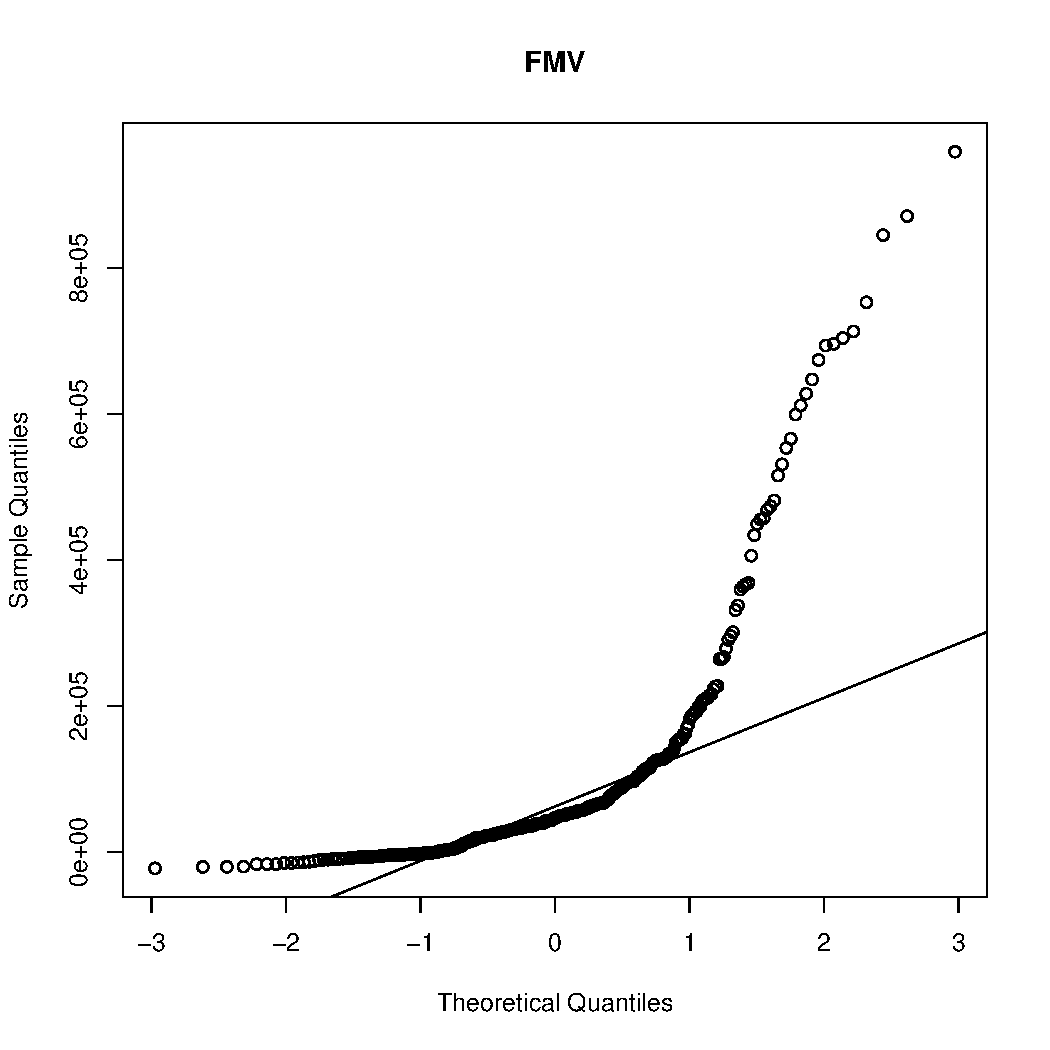
\includegraphics[width=0.6\linewidth]{figure5.pdf}
%	\caption{Overlapped Group-Lasso}
%\end{figure}
%}
\subsubsection*{Empirical results}\label{empirical_results}

The following results were computed for two independent representative portfolios of VA contracts, extracted from the synthetic data set described in Chapter~\ref{chap:dataset}. For each of them, a linear model with interactions was estimated based on the OGLASSO. The plots in Figure~\ref{original_fmv} show histograms of the FMVs as a preliminary examination of the target variable. As illustrated, the distribution is skewed to the right and there are many contracts with FMV close to zero. The QQ-plots in Figure~\ref{original_fmv} compare the theoretical distribution of the FMV (Normal) with its empirical distribution. Based on the graphical analysis it is possible to assert that the FMVs do not follow a Normal distribution, as many points on the plot are located far away from the straight line.

\begin{figure}[h!]
\makebox[\textwidth][c]{
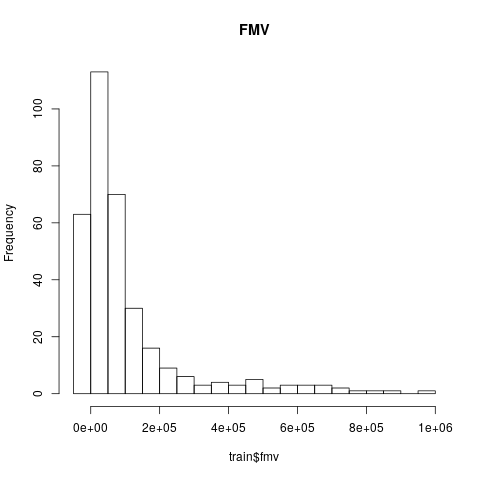
\includegraphics[scale=0.4]{pictures/original_fmv_hist_rep1}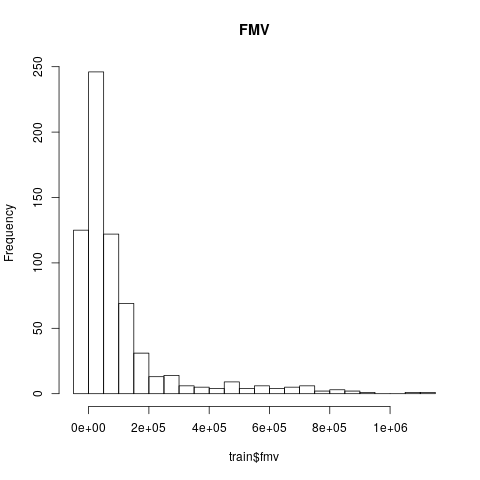
\includegraphics[scale=0.4]{pictures/original_fmv_hist_rep2} 
}
\makebox[\textwidth][c]{
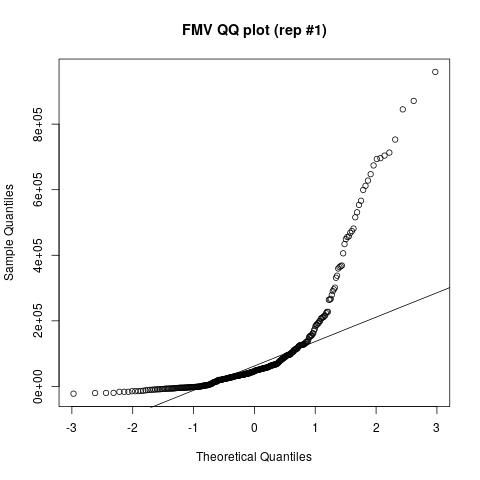
\includegraphics[scale=0.4]{pictures/boxcox_rep1_fmv_qqplot}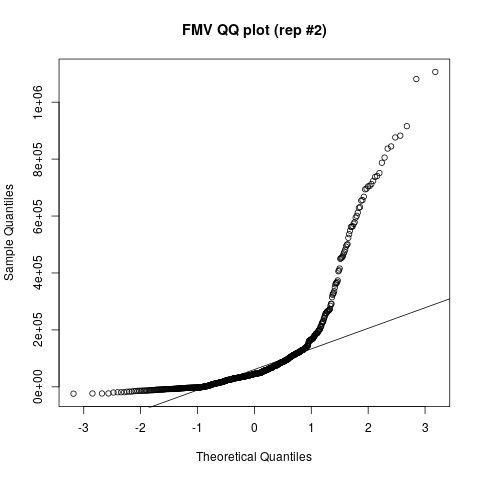
\includegraphics[scale=0.4]{pictures/boxcox_rep2_fmv_qqplot} 
}
\caption{Histograms and QQ-plots for the fair market values of the contracts in the representative portfolios.}\label{original_fmv}
\end{figure}

%After estimating the model parameters for both representative portfolios, we verify the gaussianity of the residuals. First, their histograms are illustrated in Figure~\ref{histogram_residuals_fmv}.

\begin{figure}[h!]
\makebox[\textwidth][c]{
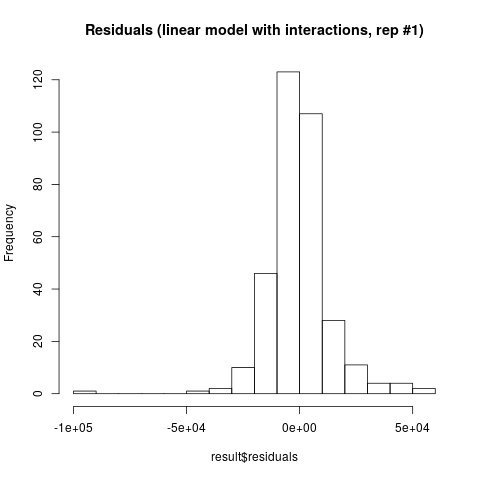
\includegraphics[scale=0.4]{pictures/original_residuals_linear_model_with_interactions_hist_rep1}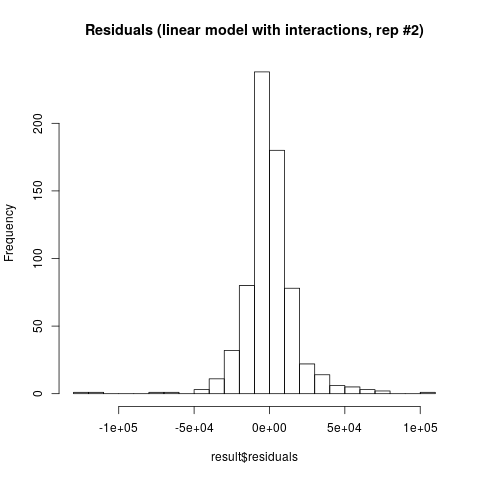
\includegraphics[scale=0.4]{pictures/original_residuals_linear_model_with_interactions_hist_rep2} 
}
\makebox[\textwidth][c]{
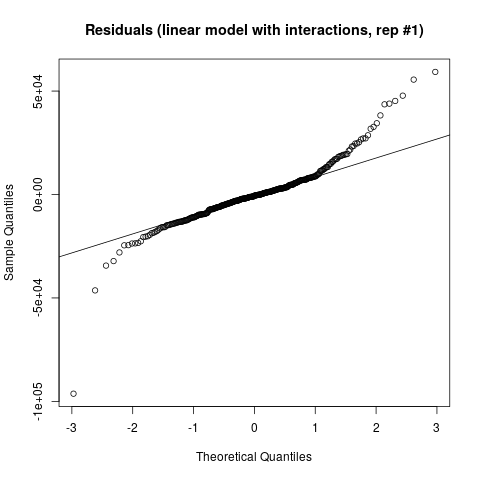
\includegraphics[scale=0.4]{pictures/original_residuals_linear_model_with_interactions_qqplot_rep1}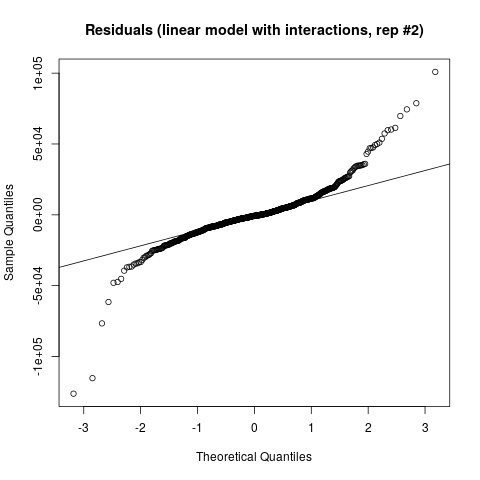
\includegraphics[scale=0.4]{pictures/original_residuals_linear_model_with_interactions_qqplot_rep2} 
}
%\caption{QQ-plots for the regression residuals for the OGLASSO models}\label{qq_plot_residuals_fmv}
\caption{Histograms and QQ-plots for the residuals of the OGLASSO models fitted for each representative portfolio.}\label{residuals_oglasso}
\end{figure}

After estimating the model parameters for both representative portfolios, we analyse the residuals of the OGLASSO models. Histograms and QQ-plots are shown in Figure~\ref{residuals_oglasso}. As expected, the residuals illustrated in the histograms are centered around zero. In addition, as the QQ-plots indicate, the residuals present heavy tails, a feature that is not consistent with the hypothesis of a Normal distribution. 
%
%The two first histograms above show the distribution of residuals after fitting the OGLASSO model, while the following two show the QQ-plot of residuals, taking the standard normal as theoretical distribution. Residuals distributed as a standard normal is a desirable property, since it is a necessary assumption to make valid inference on the estimated parameters.
%
Normally distributed residuals are a desirable feature to validate any inference built on top of the estimated parameters. As illustrated in Figure~\ref{interactions}, the statistically significant interaction terms identified for each representative portfolio are quite different.

%As residuals are clearly non-gaussian, the inference on the model is not consistent, as shown in Figure~\ref{interactions} where the significant interaction terms are illustrated.

\begin{figure}[h!]
\makebox[\textwidth][c]{
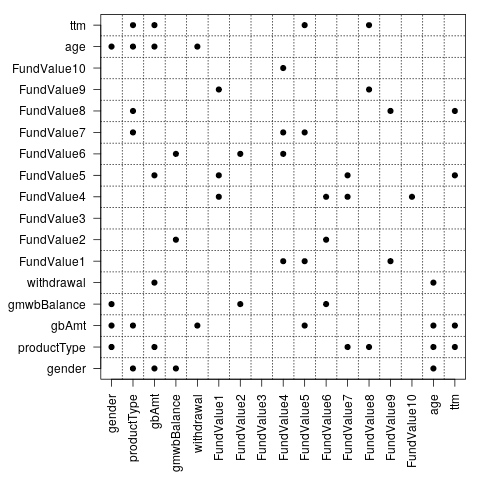
\includegraphics[scale=0.4]{pictures/original_interactions_model_rep1}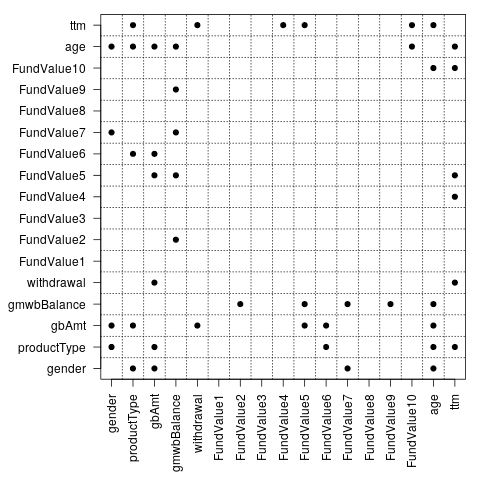
\includegraphics[scale=0.4]{pictures/original_interactions_model_rep2} 
}
\caption{Interaction matrices for the OGLASSO models, showing the statistically significant interaction terms in each model.}\label{interactions}
\end{figure}

%Analysing the last graphs, we can observe that there are some values in the tail of empirical distribution that are not fitted by a standard normal, consequently inference on the model is not consistent. 

%Despite the fact, the results show that the model is able to make good predictions of the FMV.

Despite the problems identified in the residuals of the fitted models, their predictions are quite satisfactory. These are illustrated using the QQ-plots in Figure~\ref{prediction_fmv}, where predicted FMVs are compared against their correct values. The in-sample results, computed exclusively with the contracts in the representative portfolios, give us $R^2$ values equal to 0.9928 and 0.9891 for each representative portfolio. For the full data set of VA contracts, $R^2$ values are equal to 0.9526 and 0.9618.

%The graphs above compare the model predictions for the training set and the true FMV. As closer the points are to the straight line as better is the fit in sample. 

\begin{figure}[h!]
\makebox[\textwidth][c]{
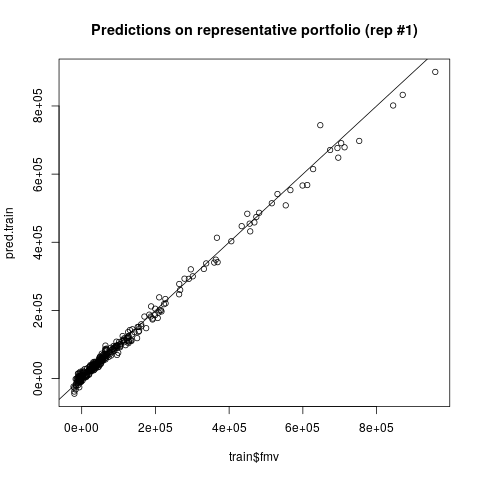
\includegraphics[scale=0.4]{pictures/original_predictions_representative_portfolio_rep1}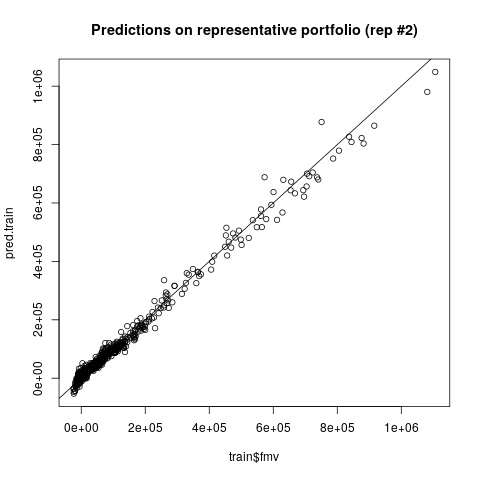
\includegraphics[scale=0.4]{pictures/original_predictions_representative_portfolio_rep2} 
}
\makebox[\textwidth][c]{
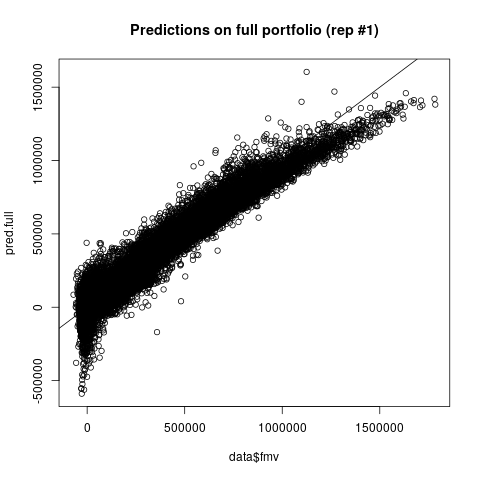
\includegraphics[scale=0.4]{pictures/original_predictions_full_portfolio_rep1}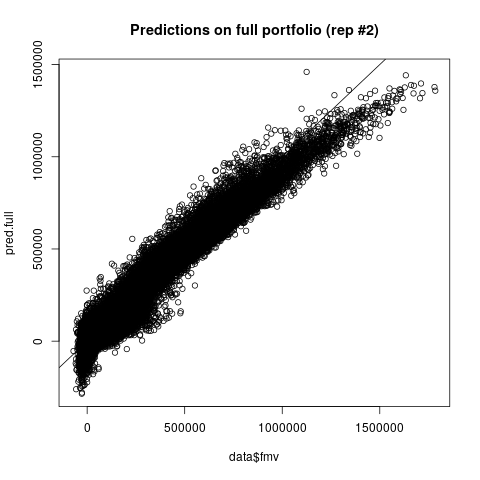
\includegraphics[scale=0.4]{pictures/original_predictions_full_portfolio_rep2} 
}
\caption{In-sample (representative portfolio) and out-of-sample (full portfolio) analysis of the predicted fair market values for VA contracts}\label{prediction_fmv}
\end{figure}

%The graphs above compare the model predictions for the training set and the true FMV. As closer the points are to the straight line as better is the fit in sample. The $r^2$ for each representative set are 0.9928 and 0.9891, respectively.
%Considering the remaining data for each representative set, the $r^2$ obtained are 0.9526 and 0.9618, respectively. The graphs bellow show the results.

% \begin{center}
% True FMV versus model predictions (training set)\\
% $r^2$: $0.9928$ and $0.9891$
% \end{center}

%In summary, the numeric results presented above show that including interaction in linear regression models is an interesting strategy to improve predictions of FMV and metamodeling process. However, as an important assumption is violated, inference based on the estimated parameters is inconsistent. In the next section, it will be discussed a transformation technique to enable consistent estimation and interpretation of parameters.

In summary, as expected, the numeric results presented above confirm that linear models with interaction terms provide excellent results for the valuation of portfolios of VA contracts. However, as an important assumption is violated, inference based on the estimated parameters is inconsistent, as illustrated in Figure~\ref{interactions}. In the next section, we discuss a technique that improves the consistency of the results.

% \begin{center}
% True FMV versus model predictions (all data)\\
% $r^2$: $0.9526$ and $0.9618$
% \end{center}

% \begin{center}
% An example with two representative portfolios:
% \end{center}

% \begin{center}
% Interactions are inconsistent!
% \end{center}


\subsection{Box-Cox regression model}

The Box-Cox transform, introduced by~\cite{box1964analysis}, is commonly used in statistics to correct the skewness and non-gaussianity of regression residuals. It is, therefore, a natural choice to improve the gaussianity of the residuals in the OGLASSO model and, consequently, improve the consistency in the significance of the interaction terms of the regression models used in the valuation of the VA portfolios.

The Box-Cox regression model is given by 

\begin{equation}
 Y(\lambda)=\beta_{0}+\beta_{1} X_{1}+\cdots+\beta_{k} X_{k}+\varepsilon,
\end{equation}
where $Y\left(\lambda \right)$ is the transformed response variable, $X_1 \ldots X_n$ the explanatory variables and $\varepsilon \sim N(0,\sigma^2)$. The transform, with parameters 
$\lambda=(\lambda_1, \lambda_2)$, is defined as 
\begin{equation}\label{boxcox}
 Y({\lambda})=\left\{\begin{array}{ll}{\frac{\left(Y+\lambda_{2}\right)^{\lambda_{1}-1}}{\lambda_{1}},} & {\text { if } \lambda_{1} \neq 0} \\ {\log \left(Y+\lambda_{2}\right),} & {\text { if } \lambda_{1}=0}\end{array}\right.
\end{equation}

As described in~\cite{box1964analysis}, the parameters $\lambda$ can be determined by maximizing the likelihood of the regression residuals. However, given the lack of appropriate software packages for the OGLASSO with the Box-Cox transform, we adopt a two-step procedure. First, we choose parameters to maximize the gaussianity of the FMVs, and then we fit the OGLASSO. Finally, we test the adequacy of the model by computing the FMVs for the entire portfolio of VA contracts, as in Section~\ref{sec:linear_model}.

The first parameter determined in our experiment is the shift $\lambda_2$, chosen to guarantee non-negative values for all transformed FMVs in the synthetic database. In the sequence,  values for $\lambda_1$ were chosen to maximize the gaussianity of the transformed FMVs in each representative portfolio. Using the estimated parameters, we found improvements in the symmetry of the transformed FMVs and also smaller deviations from the Gaussian distribution, as illustrated by the histograms and the QQ-plots in Figure~\ref{qqplot_transformed_fmv}. More importantly, after fitting the OGLASSO model for each representative portfolio, we obtain residuals that are significantly more Gaussian, as illustrated by the QQ-plots in Figure~\ref{qqplot_residuals_transformed_fmv} and their counterparts in Figure~\ref{residuals_oglasso}, where no transformations are used. 

Analysing the interaction matrices in figures~\ref{interactions} and~\ref{interactions_transformed_fmv}, we conclude that the detection of statistically significant interactions has also improved. First, we could observe an increase in the number of interactions for both representative portfolios. For the first, we notice an increased from 54 to 64 interactions, and from 46 to 76 for the second. The number of matching interactions (identified in both portfolios) has also increased, from 22 to 48. In addition, if we consider these matching interactions as correct, we also find an increase in accuracy: from 40\% to 75\% in the case of the first portfolio, and from 47\% to 63\% for the second.

The models estimated for both representative portfolios fit the transformed FMVs quite well, as their $R^2$ values are, respectively, 99.2\% and 98.6\%. In-sample predictions for the transformed FMVs and regular FMVs are illustrated in Figure~\ref{predictions_in_sample}, where they are compared against their correct values using QQ-plots. It is interesting to notice that, due to the Box-Cox transform, the transformed FMVs do not seem as concentrated as the non-transformed ones. 

We test the out-of-sample performance of the models by computing predictions for the entire data set of variable annuities. Results for both models can be found in Figure~\ref{predictions_out_of_sample}. Unfortunately, the improvements found in the in-sample results are not repeated in this test. Prediction errors are naturally larger in out-sample tests, however these seem to be inflated by the inverse Box-Cox transform, unexpectedly resulting in a poor out-of-sample performance. 

\begin{figure}[h!]
\makebox[\textwidth][c]{
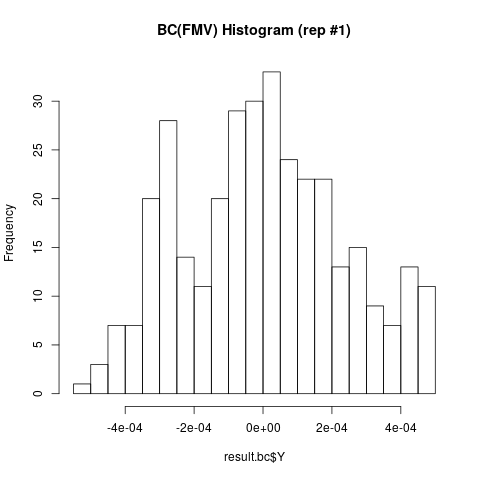
\includegraphics[scale=0.4]{pictures/boxcox_rep1_fmv_hist}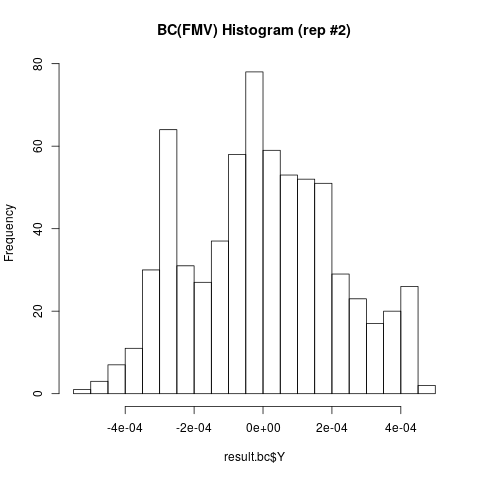
\includegraphics[scale=0.4]{pictures/boxcox_rep2_fmv_hist} 
}
\makebox[\textwidth][c]{
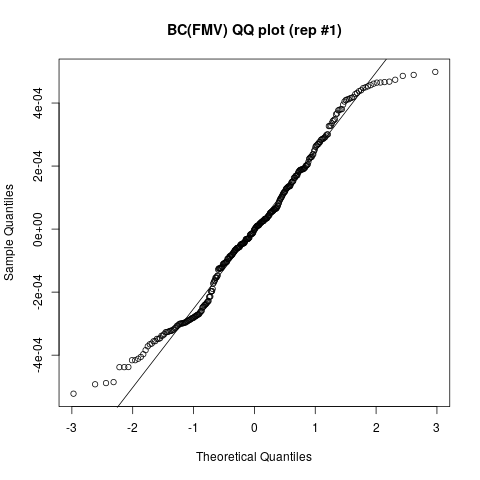
\includegraphics[scale=0.4]{pictures/boxcox_rep1_transformed_fmv_qqplot}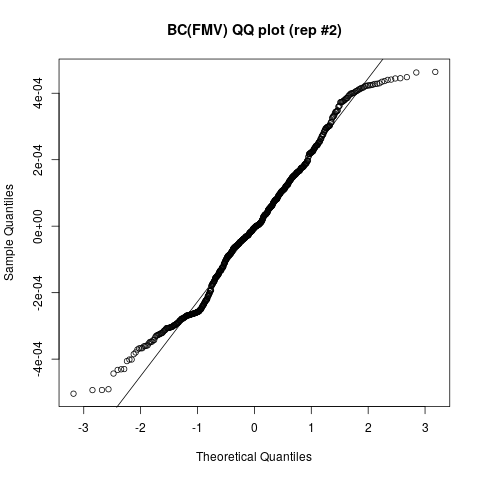
\includegraphics[scale=0.4]{pictures/boxcox_rep2_transformed_fmv_qqplot} 
}
\caption{Histograms and QQ-plots of transformed fair market values of contracts in the representative portfolios.}\label{qqplot_transformed_fmv}
\end{figure}


\begin{figure}[h!]
\makebox[\textwidth][c]{
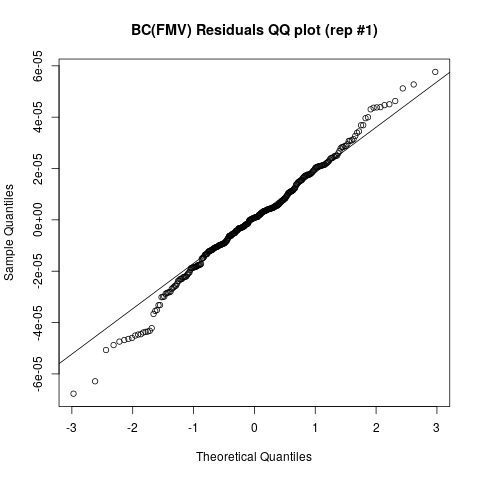
\includegraphics[scale=0.4]{pictures/boxcox_rep1_transformed_residuals_qqplot}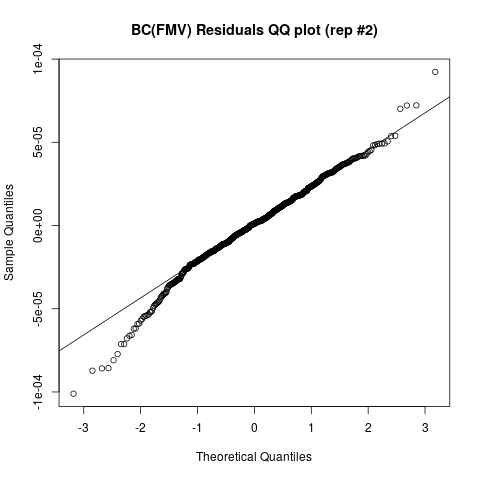
\includegraphics[scale=0.4]{pictures/boxcox_rep2_transformed_residuals_qqplot} 
}
\caption{QQ-plots of residuals for the models fitted on transformed fair market values.}\label{qqplot_residuals_transformed_fmv}
\end{figure}


\begin{figure}[h!]
\makebox[\textwidth][c]{
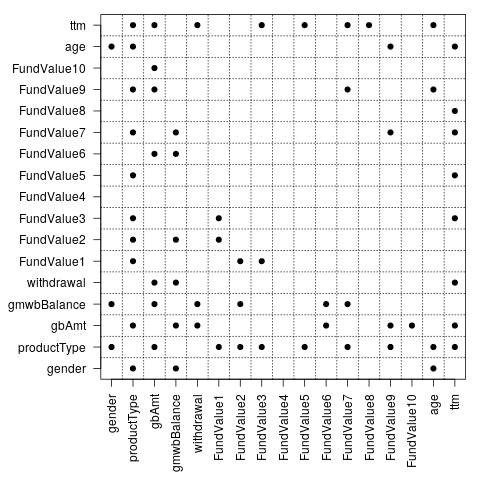
\includegraphics[scale=0.4]{pictures/boxcox_rep1_interactions}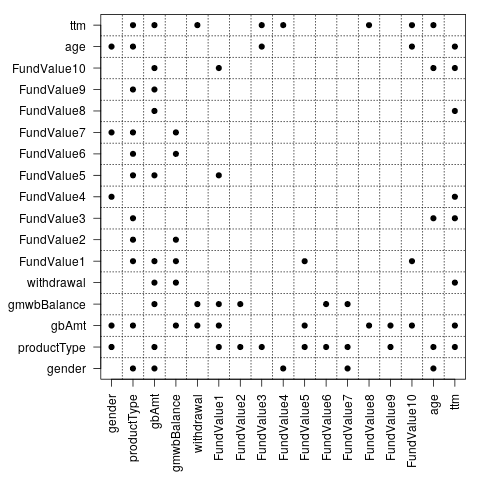
\includegraphics[scale=0.4]{pictures/boxcox_rep2_interactions} 
}
\caption{Interaction matrices for the models fitted on transformed fair market values.}\label{interactions_transformed_fmv}
\end{figure}

\begin{figure}[h!]
\makebox[\textwidth][c]{
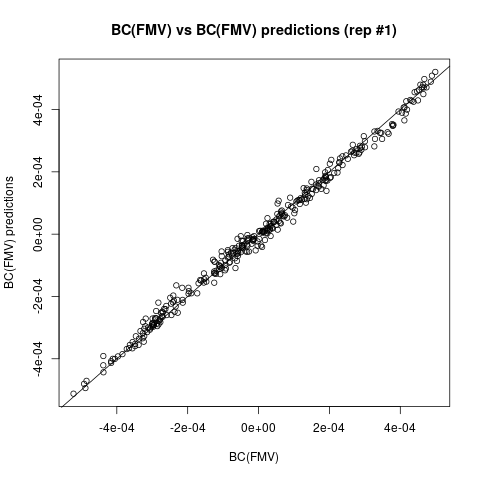
\includegraphics[scale=0.4]{pictures/boxcox_rep1_crossplot_transformed_fmv_predictions}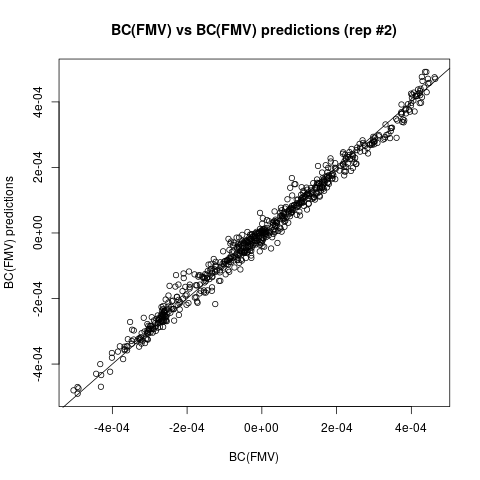
\includegraphics[scale=0.4]{pictures/boxcox_rep2_crossplot_transformed_fmv_predictions} 
}
\makebox[\textwidth][c]{
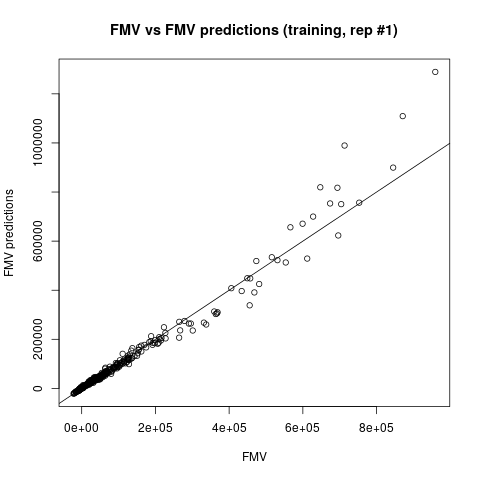
\includegraphics[scale=0.4]{pictures/boxcox_rep1_fmv_predict_train_median}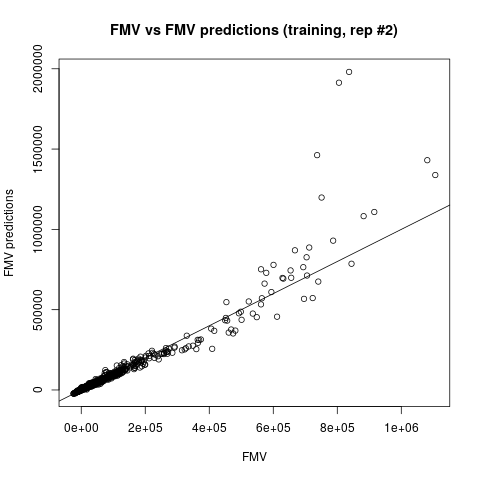
\includegraphics[scale=0.4]{pictures/boxcox_rep2_fmv_predict_train_median} 
}
%\caption{True FMV versus model predictions (training set) $r^2$: $0.9561$ and $0.8211$}\label{predictions_in_sample}
\caption{In-sample analysis of predictions for transformed fair market values (on top) and fair market values (below). The illustrated QQ-plots compare predicted values against the correct ones, available in the data set of variable annuity contracts.}\label{predictions_in_sample}
\end{figure}

\begin{figure}[h!]
\makebox[\textwidth][c]{
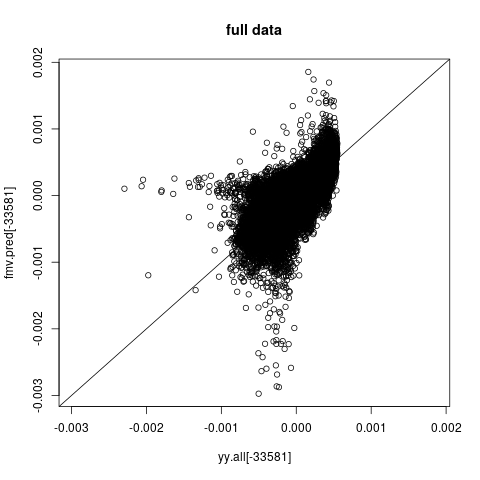
\includegraphics[scale=0.4]{pictures/boxcox_rep1_crossplot_transformed_fmv_predictions_all_data}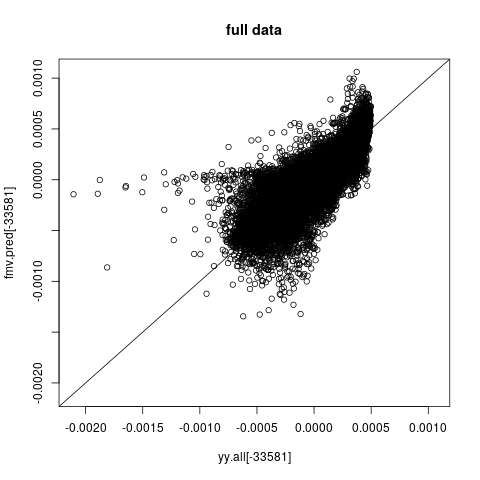
\includegraphics[scale=0.4]{pictures/boxcox_rep2_crossplot_transformed_fmv_predictions_all_data} }
%\caption{True transformed FMV versus model predictions (all data) $r^2$: $0.7788$ and $0.8616$}\label{predictions_transformed_out_of_sample}
%\end{figure}

%\begin{figure}[h!]
    \makebox[\textwidth][c]{
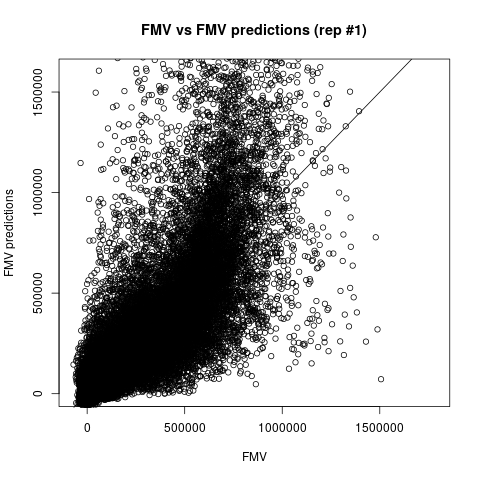
\includegraphics[scale=0.4]{pictures/boxcox_rep1_fmv_predictions_all_median}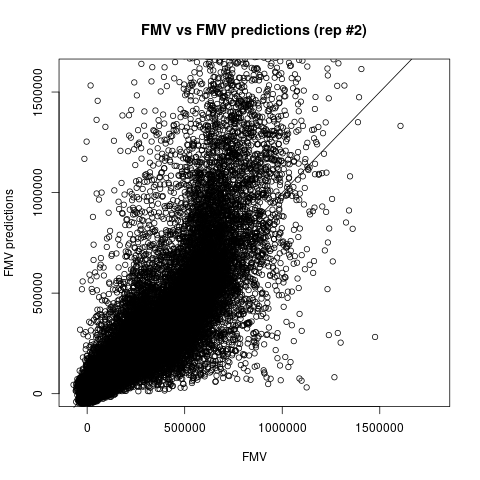
\includegraphics[scale=0.4]{pictures/boxcox_rep2_fmv_predictions_all_median} 
}
\caption{Out-of-sample analysis of predictions for transformed fair market values (on top) and fair market values (below). The illustrated QQ-plots compare predicted values against the correct ones, available in the data set of variable annuity contracts.}\label{predictions_out_of_sample}
\end{figure}


\subsection{Tree-based models}\label{sec:tree_based_models}

We also considered tree-based models as a meta-modelling approach. One advantage of these models is that they can handle categorical variables naturally, such as gender and product type. Moreover, they can capture non linear effects and interactions between variables. Other great advantages of tree-based models are their ability to perform feature selection and the fact that they are also easy to interpret by checking the tree structure.

%        \begin{itemize}
%            \item Quan, Zhiyu \& Gan, Guojun \& Valdez, Emiliano. (2018). Tree-based Models for Variable Annuity Valuation: Parameter Tuning and Empirical Analysis. SSRN Electronic Journal
%           	 \item Tree-based models can handle categorical variables naturally
%            \item Tree-based models can capture non linear effects and interactions between variables
 %           \item Tree-based models can perform feature selection
  %          \item Easy to interpret by checking the tree structure
   %     \end{itemize}



				
%To study such models we used primarily the work of quan2018treefollowing paper:
%Quan, Zhiyu \& Gan, Guojun \& Valdez, Emiliano. (2018). Tree-based Models for Variable Annuity Valuation: Parameter Tuning and Empirical Analysis. SSRN Electronic Journal.
%In this paper, the authors compare the performance of several different tree models in predicting the fair market value of VAs.

To study such models we used primarily~\cite{quan2018tree}, where the authors compare the performance of several different tree models in predicting the fair market value of VAs. As shown in Table~\ref{tab:tree}, we can see that generally, the Gradient boosting performed better. With that in mind, we focus on this method.

\begin{table}
\makebox[\textwidth][c]{
\begin{tabular}{cccccccc}
\toprule
Model & Gini & $R^2$ & CCC & ME & PE & MSE & MAE \\
\midrule
Regression tree (CART)      &  0.786    &  0.845     & 0.917    &  1.678   & -0.025   & 3278.578    & 31.421 \\
Bagged trees                & 0.842     &  0.918     & 0.954    &  2.213   & -0.033   & 1720.725    & 20.334 \\
Gradient boosting           & 0.836     &  0.942     & 0.969    &  1.311   & -0.019   & 1214.899    & 19.341 \\
Conditional inference trees & 0.824     &  0.869     & 0.930    &  0.905   & -0.013   & 2754.853    & 26.536 \\
Conditional random forests  & 0.836     &  0.892     & 0.940    &  1.596   & -0.024   & 2273.385    & 23.219 \\
Ordinary Kriging            & 0.815     &  0.857     & 0.912    & -0.812   &  0.012   & 3006.192    & 27.429 \\
GB2                         & 0.827     &  0.879     & 0.930    &  0.106   & -0.002   & 2554.246    & 27.772 \\
\bottomrule
\end{tabular}
}
\caption{Prediction accuracy of different models}\label{tab:tree}
\end{table}

%We can see that generally, the Gradient boosting performed better. With that in mind, let us look into this method more deeply:
%        \begin{itemize}
%            \item Quan, Zhiyu \& Gan, Guojun \& Valdez, Emiliano. (2018). Tree-based Models for Variable Annuity Valuation: Parameter Tuning and Empirical Analysis. SSRN Electronic Journal
%        \end{itemize}
%        \begin{figure}
% 			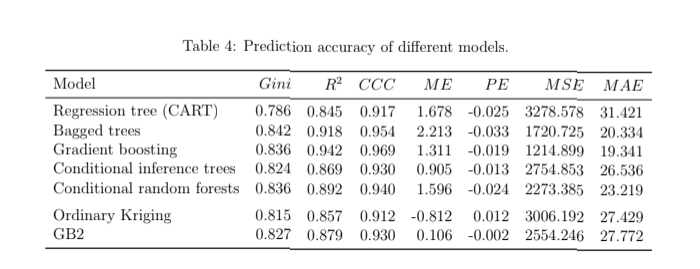
\includegraphics[width=1.0\linewidth]{pictures/emiliano_tree.png}
%   			\caption{Prediction accuracy of different models}
% 		\end{figure} 
        % inserir a imagem

%        \begin{itemize}
%			\setlength\itemsep{0,7em}
%            \item A gradient boosting regression tree is an ensemble model which grows trees by sequentially putting more weights on residuals of previous trees
 %           \item The final tree is given by:
  %          $$f_{B}(\mathbf{X})=\sum_{b=1}^{B} T_{b}\left(\mathbf{X} ; \Theta_{b}\right)$$
   %      	\item where $T_{b}\left(\mathbf{X} ; \Theta_{b}\right)$ are the regression trees. $B$ is the number of iterations or the number of additive trees. In each step $b,$ for $b=1, \ldots, B,$ we need to find the regression $\Theta_{b}$ based on
%the following optimization problem:
%
 %        	$$\hat{\Theta}_{b}=\underset{\Theta_{b}}{\arg \min } \sum_{i=1}^{N} L\left(y_{i}, f_{b-1}\left(\mathbf{X}_{i}\right)+T_{b}\left(\mathbf{X}_{i} ; \Theta_{b}\right)\right)$$
         	
  %      \end{itemize}

A gradient boosting regression tree is an ensemble model which grows trees by sequentially putting more weights on residuals of previous trees. The final tree is given by:    
$$f_{B}(\mathbf{X})=\sum_{b=1}^{B} T_{b}\left(\mathbf{X} ; \Theta_{b}\right)$$
where $T_{b}\left(\mathbf{X} ; \Theta_{b}\right)$ are the regression trees, and $B$ is the number of iterations or the number of additive trees. In each step $b,$ for $b=1, \ldots, B,$ we need to find the regression $\Theta_{b}$ based on the following optimization problem:
	$$\hat{\Theta}_{b}=\underset{\Theta_{b}}{\arg \min } \sum_{i=1}^{N} L\left(y_{i}, f_{b-1}\left(\mathbf{X}_{i}\right)+T_{b}\left(\mathbf{X}_{i} ; \Theta_{b}\right)\right)$$
%        \begin{itemize}
%        	\setlength\itemsep{0,7em}
%            \item GBM using 1000 trees and maximum depth = 3
%            \item training for 100 random sets of representatives VAs, each containing 340 contracts
%            \item The error measure are smaller for the overlapped grouped lasso model
%            \item The error measures vary a lot more for the GBM tree model then for the overlapped grouped lasso model, suggesting that the former is more robust to the selection of the representative contracts
%        \end{itemize}
Being that the gradient boosting regression tree was the best model for our case, we wanted to compare its performance against the overlapped group lasso model, which had very good results, as shown in Section~\ref{sec:linear_model}. Furthermore, we wished to test the robustness of each model to the set of representative contracts. In order to do so, we trained each model with 100 random sets of representative VAs, each containing 340 contracts. We used 100 trees and maximum depth of 3 for the GBM. 
%The results follow below:
As the tables~\ref{gbm_erros} and~\ref{lasso_erros} show, the error measures are smaller for the overlapped grouped lasso model. Additionally, the error measures vary a lot more for the GBM tree model then for the overlapped grouped lasso model, suggesting that the former is more robust to the selection of the representative contracts.

\begin{table}[ht]
\centering
\begin{tabular}{rrrrrr}
\toprule
 & $|$PE$|$ & R2 & $|$ME$|$ & MAE & MSE \\
\midrule
%Rep. VAs: 340 & 0.17 & 0.74 & 16.95 & 57.85 & 7542.90 \\
  %Rep. VAs: 680 & 0.04 & 0.73 & 3.90 & 57.43 & 7809.42 \\
  Min. & 0.00 & 0.87 & 0.00 & 28.46 & 2180.66 \\
  1st Qu. & 0.01 & 0.89 & 1.41 & 30.72 & 2517.63 \\
  Median & 0.03 & 0.90 & 2.66 & 31.63 & 2776.60 \\
  Mean & 0.03 & 0.90 & 2.80 & 31.91 & 2822.27 \\
  3rd Qu. & 0.04 & 0.91 & 3.82 & 33.00 & 3053.23 \\
  Max. & 0.10 & 0.92 & 9.37 & 36.60 & 3858.51 \\
\bottomrule
\end{tabular}
\caption{GBM Tree: Error measures for multiple sets of representatives contracts}
\label{gbm_erros}
\end{table}

\begin{table}[ht]
\centering
\begin{tabular}{rrrrrr}
\toprule
 & $|$PE$|$ & R2 & $|$ME$|$ & MAE & MSE \\
\midrule
%Rep. VAs: 340 & 0.01 & 0.95 & 0.87 & 23.29 & 1377.79 \\
 %Rep. VAs: 680 & 0.01 & 0.96 & 1.16 & 20.89 & 1104.23 \\
  Min. & 0.00 & 0.93 & 0.08 & 18.59 & 810.84 \\
  1st Qu. & 0.00 & 0.96 & 0.40 & 20.79 & 1074.65 \\
  Median & 0.01 & 0.96 & 1.09 & 21.28 & 1163.91 \\
  Mean & 0.01 & 0.96 & 1.31 & 21.33 & 1182.15 \\
  3rd Qu. & 0.02 & 0.96 & 1.82 & 21.88 & 1248.26 \\
  Max. & 0.05 & 0.97 & 4.79 & 23.70 & 1911.56 \\
\bottomrule
\end{tabular}
\caption{Overlapped Group Lasso: Error measures for multiple sets of representatives contracts}
\label{lasso_erros}
\end{table}	


%\chapter{Neural network}

		\begin{itemize}
			\setlength\itemsep{0,5em}
			\item In Heajzi and Jackson (2016), the authors proposed a neural network apporach with only one hidden layer and feed-foward approximation to calculate distance function.
			\item Extended version of the Nadaraya-Watson kernel regression model to estimate the Greeks: Assuming $y\left(z_{1}\right), \cdots, y\left(z_{n}\right)$  are  the observed values at known locations $z_{1}, \cdots, z_{n}$ the Nadaraya-Watson estimator approximates the value $y(z)$ at the location $z$ by:
		\end{itemize}			 			 
		\begin{equation}
\hat{y}(z)=\sum_{i=1}^{n} \frac{K_{h}\left(z-z_{i}\right) \times y\left(z_{i}\right)}{\sum_{j=1}^{n} K_{h}\left(z-z_{j}\right)}
		\end{equation}
		
		\;\;\;\;\;\;\centering where $K_h$ is a kernel with a bandwidth of $h$.
		 
		\begin{itemize}
			\setlength\itemsep{0,5em}
			\item The Nadaraya-Watson estimator was first proposed for kernel regression applications and hence the choice of kernel function $K_h$ was a necessity.  For our application of interest, we choose to use the following extended version of the Nadaraya-Watson estimator:
		\end{itemize}			 			 
		\begin{equation}
\hat{y}(z)=\sum_{i=1}^{n} \frac{G_{h_{i}}\left(z-z_{i}\right) \times y\left(z_{i}\right)}{\sum_{j=1}^{n} G_{h_{j}}\left(z-z_{j}\right)}
		\end{equation}
		
		\;\;\;\;\;\;\centering where $G$ is a nonlinear differentiable function and the subscript $h_i$, similar to the bandwidth $h$ of kernels, denotes the range of influence of each $y(z_i)$ on  the  estimated  value.
		 
		\begin{itemize}
			\setlength\itemsep{0,5em}
			\item Assuming $x_1,···,x_n$ are the inputs of neuron $j$ at hidden levell.  First a linear combination of input variables is constructed at each neuron:
		\end{itemize}			 			 
		\begin{equation}
		a_{j}^{(l)}=\sum_{i=1}^{n} w_{i j}^{(l)} x_{i}+b_{j}^{(l)}
		\end{equation}
		
		\;\;\;\;\;\;\centering where parameters $w_{ij}$ are referred to as weights and parameter $b_j$ is called the bias.
		 
		\begin{itemize}
			\setlength\itemsep{0,5em}
			\item Our proposed neural network allows us to rewrite Equation (1) as:
		\end{itemize}			 			 
		\begin{equation}
		\hat{y}(z)=\sum_{i=1}^{n} \frac{\exp \left(\mathbf{w}_{\mathbf{i}}^{T} \mathbf{f}\left(z, z_{i}\right)+b_{i}\right) \times y\left(z_{i}\right)}{\sum_{j=1}^{n} \exp \left(\mathbf{w}_{\mathbf{j}}^{T} \mathbf{f}\left(z, z_{j}\right)+b_{j}\right)}
		\end{equation}
		
		\;\;\;\;\;\;\centering where the vector $f(z,z_i)$ represents the features in the input layer that are related to the representative VA policy $z_i$, and vector $w_i$ contains the weights associated with each feature in $f$ at neuron $i$ of the hidden layer. 
		 
		\begin{itemize}
			\setlength\itemsep{0,5em}
			\item Those features $f(z,z_i)$ behave in different ways if variable $z_i$ is categorical or continuous. If it is categorical then we have:
		\end{itemize}			 			 
		\begin{equation}
		f(z,z_i)=\left\{\begin{array}{ll}{0} & {\text { if } x_{c}=x_{c_{i}}} \\ {1} & {\text { if } x_{c} \neq x_{c_{i}}}\end{array}\right.
		\end{equation}
		\begin{itemize}
			\setlength\itemsep{0,5em}
			\item  If it is continuous then we have:
		\end{itemize}			 			 
		\begin{equation}
		f\left(z, z_{i}\right)=\frac{\left[t(x)-t\left(x_{i}\right)\right]^{+}}{R_{t}}
		\end{equation}
		
		\centering $t \in\{\text { maturity, age }, \mathrm{AV}, \mathrm{GD} / \mathrm{AV}, \mathrm{GW} / \mathrm{AV}, \text { withdrawal rate }\}$
		 
		\begin{itemize}
			\setlength\itemsep{0,5em}
			\item The objective of the calibration process is then to find a set of weights and bias parameters that minimizes the Mean Squared Error (MSE) in the estimation of the Greeks of the training portfolio. 
		\end{itemize}			 			 
		\begin{equation}
		E(\mathbf{w}, \mathbf{b})=\frac{1}{2|B|} \sum_{k=1}^{|B|}\left\|\hat{y}\left(\overline{z}_{k}, \mathbf{w}, \mathbf{b}\right)-y\left(\overline{z}_{k}\right)\right\|^{2}
		\end{equation}
		
		\;\;\;\;\;\;\centering where $\overline{z}_{k}, 1 \leq k \leq|B|,$ are the VA policies in the training portfolio.
		 

%\chapter{Conclusion}





%\chapter{Introduction} \input{Chapters/"Introduction"/"Introduction"}
%\newpage
%\chapter{Literature} \input{Chapters/"Literature"/"Literature"}
%\newpage
%\chapter{Synthetic Data} \input{Chapters/"Synthetic Data"/"Synthetic Data"}
%\newpage
%\chapter{Metamodeling Approach} \input{Chapters/"Metamodeling Approach"/"Metamodeling Approach"}
%\newpage
%\chapter{Conclusion} \input{Chapters/"Conclusion"/"Conclusion"}

	
\newpage
\bibliographystyle{elsarticle-harv}
%\bibliographystyle{plain}
%\bibliography{BibliographySample}
%GAN, Guojun. Application of metamodeling to the valuation of large variable annuity portfolios. In: Proceedings of the 2015 Winter Simulation Conference. IEEE Press, 2015. p. 1103-1114.

%GAN, Guojun; VALDEZ, Emiliano A. Regression modeling for the valuation of large variable annuity portfolios. North American Actuarial Journal, v. 22, n. 1, p. 40-54, 2018.

%GAN, Guojun; VALDEZ, Emiliano A. Modeling partial greeks of variable annuities with dependence. Insurance: Mathematics and Economics, v. 76, p. 118-134, 2017.

%GAN, Guojun. Valuation of large variable annuity portfolios using linear models with interactions. Risks, v. 6, n. 3, p. 71, 2018.

%GAN, Guojun; VALDEZ, Emiliano A. Metamodeling for Variable Annuities. CRC Press, 2019.

%GAN, Guojun; VALDEZ, Emiliano A. Valuation of Large Variable Annuity Portfolios with Rank Order Kriging. North American Actuarial Journal, Forthcoming, 2019.

%HEJAZI, Seyed Amir; JACKSON, Kenneth R.; GAN, Guojun. A spatial interpolation framework for efficient valuation of large portfolios of variable annuities. arXiv preprint arXiv:1701.04134, 2017.

%HEJAZI, Seyed Amir. A Neural Network Approach to Efficient Valuation of Large VA Portfolios. 2016. Phd thesis. University of Toronto (Canada).

%XU, Wei et al. Moment matching machine learning methods for risk management of large variable annuity portfolios. Journal of Economic Dynamics and Control, v. 87, p. 1-20, 2018  
%\newpage

%\bibliographystyle{plain}
%\bibliography{sp}
%\bibliographystyle{amsplain}
%\addcontentsline{toc}{section}{References}
\bibliography{reference}

\end{document}